\chapter[The 5$^{\text{th}}$ of April 2024 - Mixed formulation, orthogonalisation \& mor]{Mixed formulation, orthogonalisation \& more}


\begin{chapabstract}
	No meeting but note of ideas and discussions
\end{chapabstract}


\minitoc

\section{Mixed formulation}

\begin{itemize}
	\item LATIN the return?
	\begin{itemize}
		\item Play with the weight of the PDE and CRE terms in the loss to alternate between solving the pde or the constitutive relation
	\end{itemize}
\end{itemize}

\section{Parametrisation}

\subsection{Orthogonality}
\begin{itemize}
	\item GS does not help, somehow hard to cancel out modes (b puting them to zero or the parameters modes associated with them) hence better to juste have redundant good modes than orthogonal noise
	\begin{itemize}
		\item Put the orthogonalisation outside of forward as the forward function is not called during the training
	\end{itemize}
\end{itemize}

\subsection{Parametrisation}

\begin{itemize}
	\item With the level-set functions isn't there risk with parameters that do not play a role away from the boundary in the TD?
	\item Might also be hard to generate training scenarios (not all combination of parameters would make sense comparer with more standard parametrisation)
\end{itemize}


\subsection{PGD}

\begin{itemize}
	\item How to get a greedy algorithm without loosing the momentum of the optimiser (changing the architecture)
	\begin{itemize}
		\item Set $N$ modes, the max number of modes
		\item Unfreeze only the $n$ first modes and use only them in the loss
		\item Gradually increase $n$
	\end{itemize}
\end{itemize}



\Rq{\begin{itemize}
		\item Directly setting $n$ as trainable is not possible
		\begin{itemize}
			\item  Rely on L1 reguarisation to force the last modes to go to zero and compute $n$ as last significant mode before computing the loss
			\item Or have a set training strategy based on the loss decay (as classically done with PGD)
		\end{itemize}
	\end{itemize}
}

\Rqs{Not optimal in term of memory usage: stores a lot of zeros, but should be ok computationally-wise as only $n$ modes are used to compute the loss.}{For some reason even with a low number of trainable parameters and only the first $n$ modes being used to compute the loss (and therefore its gradient) having a higher $N$ leads to significantly slower execution. This has to be investigated, maybe it will be required to change the architecture to gradually increase the size of the HiDeNN but that would also mean losing the momentum of the optimiser each time a mode is added.}


\subsubsection{Criterion for mode addition}

In order to choose whether or not to add a mode, a criterion has to be chosen.

\begin{figure}
	\begin{subfigure}[t]{0.5\linewidth}
		\centering
		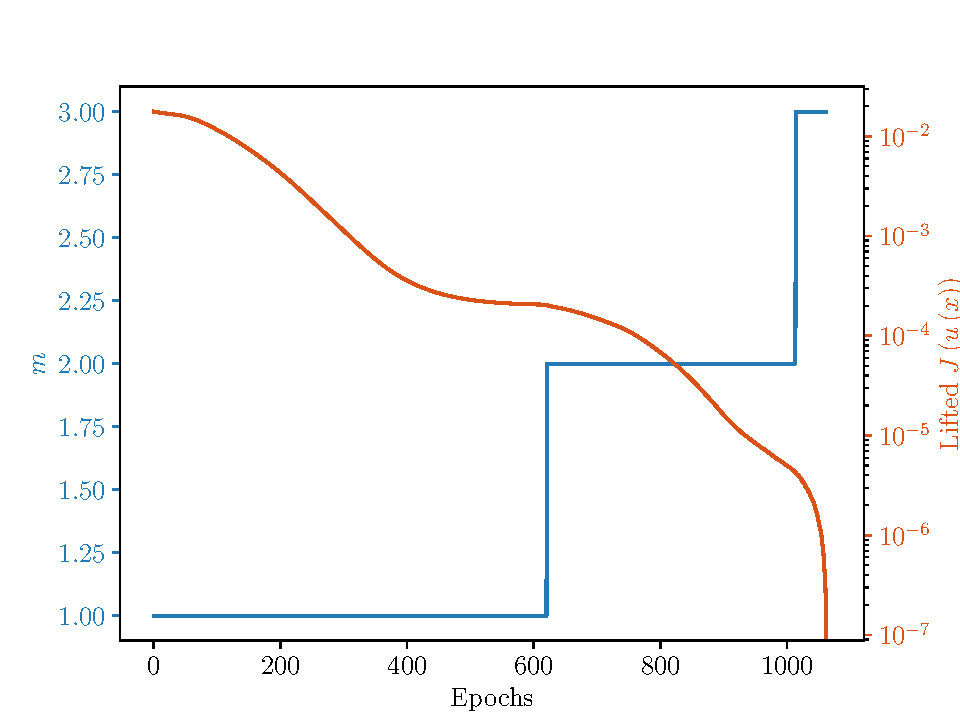
\includegraphics[width=\linewidth]{Figures/Loss_Modes.pdf}
		\caption{Loss decay and mode evolution}
	\end{subfigure}
	\begin{subfigure}[t]{0.5\linewidth}
		\centering
		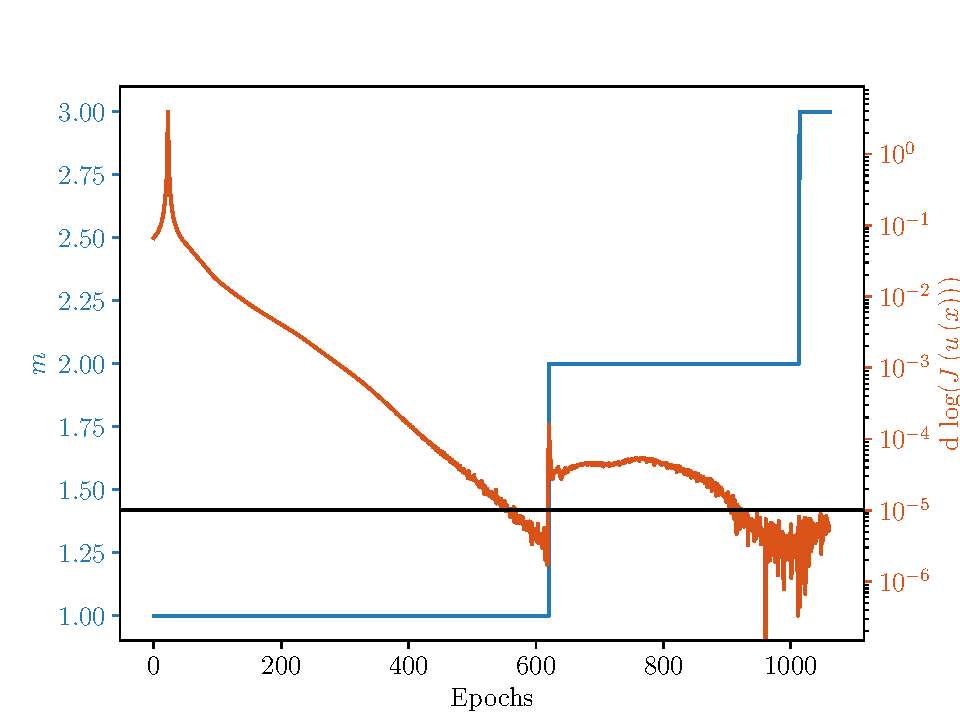
\includegraphics[width=\linewidth]{Figures/LossDecay_Modes.pdf}
		\caption{Loss logarithmic derivative and mode evolution}
	\end{subfigure}  
	\caption{Choice of the mode addition criterion}
	\label{fig:Criterion_mode}
\end{figure}

\Rqs{Because we are looking at the lifted J, the very small decade crossing at the end are visible but do not appear in the derivation that is computed on the actual J and not the lifeted version (as the minimum is only known at the end of the minisation process)}{This is very visible when comparing error and lifted energy, see \cref{fig:Impact_lift}. We do not plot the energy but the energy error that tends to 0. But the derivative is computed on the energy... We need an \emph{a priori} error estimator that tends to 0 (that omit discretisation error for instance. Is is the case with the residual error given by the mixed formulation?)}

\begin{figure}
	\begin{subfigure}[t]{0.5\linewidth}
		\centering
		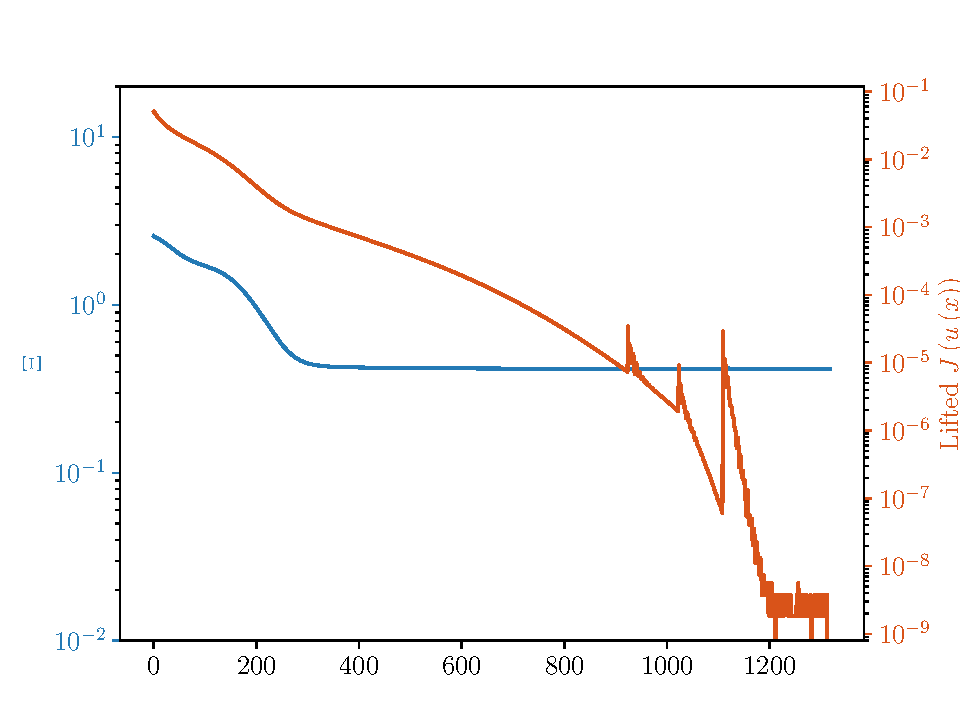
\includegraphics[width=\linewidth]{Figures/Loss_Error_Modes_Mono_1.pdf}
		\caption{Lifted loss and real L2 error}
	\end{subfigure}
	\begin{subfigure}[t]{0.5\linewidth}
		\centering
		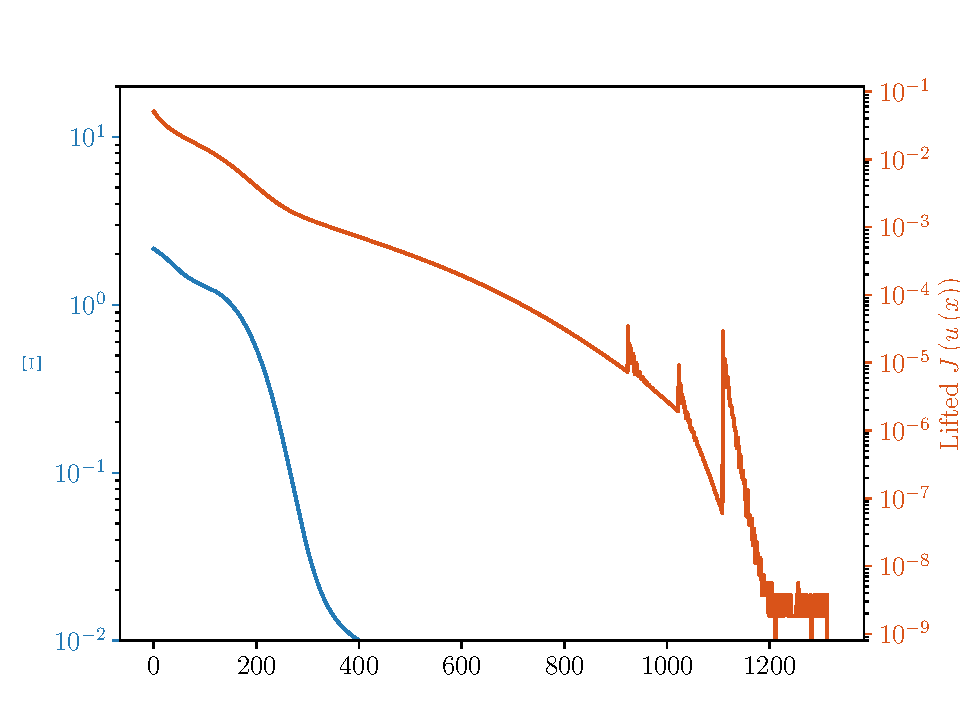
\includegraphics[width=\linewidth]{Figures/Loss_Error_Modes_Mono_2.pdf}
		\caption{Lifted loss and L2 error}
	\end{subfigure}  
	\caption{Impact of lifting}
	\label{fig:Impact_lift}
\end{figure}
